\documentclass[12pt,letterpaper]{article}
\usepackage{graphicx,textcomp}
\usepackage{natbib}
\usepackage{setspace}
\usepackage{fullpage}
\usepackage{color}
\usepackage[reqno]{amsmath}
\usepackage{amsthm}
\usepackage{fancyvrb}
\usepackage{amssymb,enumerate}
\usepackage[all]{xy}
\usepackage{endnotes}
\usepackage{lscape}
\newtheorem{com}{Comment}
\usepackage{float}
\usepackage{hyperref}
\newtheorem{lem} {Lemma}
\newtheorem{prop}{Proposition}
\newtheorem{thm}{Theorem}
\newtheorem{defn}{Definition}
\newtheorem{cor}{Corollary}
\newtheorem{obs}{Observation}
\usepackage[compact]{titlesec}
\usepackage{dcolumn}
\usepackage{tikz}
\usetikzlibrary{arrows}
\usepackage{multirow}
\usepackage{xcolor}
\newcolumntype{.}{D{.}{.}{-1}}
\newcolumntype{d}[1]{D{.}{.}{#1}}
\definecolor{light-gray}{gray}{0.65}
\usepackage{url}
\usepackage{listings}
\usepackage{color}

\definecolor{codegreen}{rgb}{0,0.6,0}
\definecolor{codegray}{rgb}{0.5,0.5,0.5}
\definecolor{codepurple}{rgb}{0.58,0,0.82}
\definecolor{backcolour}{rgb}{0.95,0.95,0.92}

\lstdefinestyle{mystyle}{
	backgroundcolor=\color{backcolour},   
	commentstyle=\color{codegreen},
	keywordstyle=\color{magenta},
	numberstyle=\tiny\color{codegray},
	stringstyle=\color{codepurple},
	basicstyle=\footnotesize,
	breakatwhitespace=false,         
	breaklines=true,                 
	captionpos=b,                    
	keepspaces=true,                 
	numbers=left,                    
	numbersep=5pt,                  
	showspaces=false,                
	showstringspaces=false,
	showtabs=false,                  
	tabsize=2
}
\lstset{style=mystyle}
\newcommand{\Sref}[1]{Section~\ref{#1}}
\newtheorem{hyp}{Hypothesis}

\title{Problem Set 1}
\date{Due: September 30, 2024}
\author{Applied Stats/Quant Methods 1}

\begin{document}
	\maketitle
	
	\section*{Instructions}
	\begin{itemize}
	\item Please show your work! You may lose points by simply writing in the answer. If the problem requires you to execute commands in \texttt{R}, please include the code you used to get your answers. Please also include the \texttt{.R} file that contains your code. If you are not sure if work needs to be shown for a particular problem, please ask.
\item Your homework should be submitted electronically on GitHub.
\item This problem set is due before 23:59 on Monday September 30, 2024. No late assignments will be accepted.
%\item Total available points for this homework is 80.
	\end{itemize}
	
	\vspace{1cm}
	\section*{Question 1: Education}

A school counselor was curious about the average of IQ of the students in her school and took a random sample of 25 students' IQ scores. The following is the data set:\\
\vspace{.5cm}

\lstinputlisting[language=R, firstline=36, lastline=36]{PS01.R}  

\vspace{1cm}

\begin{enumerate}
	\item Find a 90\% confidence interval for the average student IQ in the school.\\
	
	\item Next, the school counselor was curious  whether  the average student IQ in her school is higher than the average IQ score (100) among all the schools in the country.\\ 
	
	\noindent Using the same sample, conduct the appropriate hypothesis test with $\alpha=0.05$.
\end{enumerate}
\newpage
\section*{Solution 1: Education}

\vspace{3mm}
\begin{enumerate}
    \item \textit{Solution for Part 1}
    
       \begin{figure}[h]
              \centering
              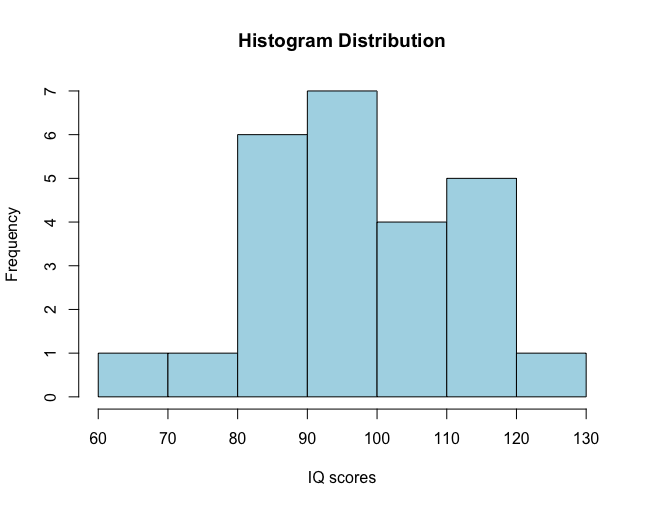
\includegraphics[width=0.5\linewidth]{images/histogram_plot.png}
              \caption{Histogram plot}
          \end{figure}
    
    We use the formula for computing the confidence interval
            \[ CI = (\bar{x} – EBM, \bar{x} + EBM) \]

       where EBM = 
        \[ EBM =  t_(\left(\frac{\alpha}{2}, df=24\right)) \times \left(\frac{s}{sqrt(n)}\right) \]

    We will use the \textit{t-distribution} in the above case as we have:

        \begin{enumerate}
          \item n \textless 30
          \item standard deviation of the population is unknown
          \item the data is approximately normally distributed as shown in Figure 1
        \end{enumerate}


    To find the critical t value, we will compute alpha/2 and degrees of freedom from the t distribution table. 

        alpha = 1 - Confidence Interval = 1 - 0.90 
        
        alpha/2 = 0.10/2 = 0.05

        degrees of freedom = n - 1 = 25 - 1 = 24

    Using the above values of alpha and degrees of freedom, the t-value becomes: 1.71 (from the t-distribution table, calculated in R)

    Given the standard deviation $s$ = 13.09 (computed from the data) and n = 25, $\bar{x} = 98.44$ , the confidence intervals become

    where, 

    upper bound for the mean = 
    \[ 98.44 + 1.71 \times \left(\frac{13.09}{\sqrt{25}}\right) \] = \textbf{102.92} \\
    lower bound for the mean = 
    \[ 98.44 - 1.71 \times \left(\frac{13.09}{\sqrt{25}}\right) \] = \textbf{93.95}

  Therefore, we can say with \textbf{90\% confidence} that the mean lies within the range of \textbf{93.95 and 102.92}
\vspace{3mm}

Code for computing the above: 

\begin{lstlisting}[language=R]

y <- c(105, 69, 86, 100, 82, 111, 104, 110, 87, 108, 87, 90, 94, 113, 112, 98, 80, 97, 95, 111, 114, 89, 95, 126, 98)

### histogram to check if normally distributed
hist(y, col = "lightblue", main = "Histogram Distribution", xlab = "IQ scores")

## finding input parameters for computing confidence intervals

length_y <- length(y)
sample_mean <- mean(y)
sample_std_dev <- sd(y)
alpha <- 1 - 0.90 
alpha_by_2 <- alpha/2 ## as confidence interval is a two tail test

## calculate t critical value and error bounds

t <- qt(1 - (alpha_by_2), df = length_y - 1)
error_bound <- t * (sample_std_dev/sqrt(length_y))

## upper and loewr bounds for confidence intervals

upper_error_bound <- sample_mean + error_bound
lower_error_bound <- sample_mean - error_bound
\end{lstlisting}
\vspace{3mm}
\item Solution for part 2

\vspace{3mm}

For this problem, our null hypothesis $H_0$ and alternative hypothesis $H_a$ are as follows:

\begin{itemize}
    \item $H_0$: $\mu \leq 100$
    \item $H_a$: $\mu \textgreater 100$
\end{itemize}

Since, $\mu$ falls on only one side, we are going to use a one tail test, or in this case a right sided one-tail test. Additionally, since the below two conditions are met we are going to use the t test to reject or accept the null hypothesis. 

       \begin{enumerate}
          \item n \textless 30
          \item standard deviation of the population is unknown
        \end{enumerate}


We are going to perform the hypothesis test using the following steps:

\begin{itemize}
    \item Step 1: Compute the t critical value \\
    With $alpha = 0.05$ and degrees of freedom = 24, the t critical value = 1.71. 
    
    \item Step 2: Compute the t-statistic value. \\ 
  
    To compute this, we use the formula: 

    \[\frac{\bar{x} - \mu_0}{s/\sqrt(n)}\]

    where,
    sample mean $\bar{x} = 98.44$, \\
    sample std dev, $s = 13.09$, \\
    hypothesized mean, $\mu_0 = 100$ and \\
    length of y, $n = 25$ \\

    the t statistic value therefore equals = -0.595

    \item Step 3: Compare the two values to accept or reject the hypothesis. \\ 
    
    Since the t critical value is greater than the t statistic value, we do not reject the null hypothesis. Therefore, we cannot say with 95\% confidence that our average student IQ is higher than 100.
    
\end{enumerate}

Code for above computations:

\begin{lstlisting}[language=R]
hypothesized_mean = 100
alpha_2 = 0.05 
t_value = (sample_mean - hypothesized_mean) / (sample_std_dev / sqrt(length_y))

# we use 1 - alpha as this is a one-tail test

t_critical = qt(1 - alpha_2, df = length_y - 1)

if (t_value > t_critical) {
  print("Reject the null hypothesis in favor of the alternative hypothesis")
} else {
  print("Do not reject the null hypothesis.")
        }
\end{lstlisting}

\end{enumerate}
\newpage
	\section*{Question 2: Political Economy}

\noindent Researchers are curious about what affects the amount of money communities spend on addressing homelessness. The following variables constitute our data set about social welfare expenditures in the USA. \\
\vspace{.5cm}


\begin{tabular}{r|l}
	\texttt{State} &\emph{50 states in US} \\
	\texttt{Y} & \emph{per capita expenditure on shelters/housing assistance in state}\\
	\texttt{X1} &\emph{per capita personal income in state} \\
	\texttt{X2} &  \emph{Number of residents per 100,000 that are "financially insecure" in state}\\
	\texttt{X3} &  \emph{Number of people per thousand residing in urban areas in state} \\
	\texttt{Region} &  \emph{1=Northeast, 2= North Central, 3= South, 4=West} \\
\end{tabular}

\vspace{.5cm}
\noindent Explore the \texttt{expenditure} data set and import data into \texttt{R}.
\vspace{.5cm}
\lstinputlisting[language=R, firstline=54, lastline=54]{PS01.R}  
\vspace{.5cm}
\begin{itemize}

\item
Please plot the relationships among \emph{Y}, \emph{X1}, \emph{X2}, and \emph{X3}? What are the correlations among them (you just need to describe the graph and the relationships among them)?
\vspace{.5cm}
\item
Please plot the relationship between \emph{Y} and \emph{Region}? On average, which region has the highest per capita expenditure on housing assistance?
\vspace{.5cm}
\item
Please plot the relationship between \emph{Y} and \emph{X1}? Describe this graph and the relationship. Reproduce the above graph including one more variable \emph{Region} and display different regions with different types of symbols and colors.
\end{itemize}

\newpage

\section*{Solution 1: Political Economy}

\begin{enumerate}
    \item Part 1

    


  \begin{figure}[h]
     \centering
       \begin{minipage}{.5\textwidth}
         \centering
           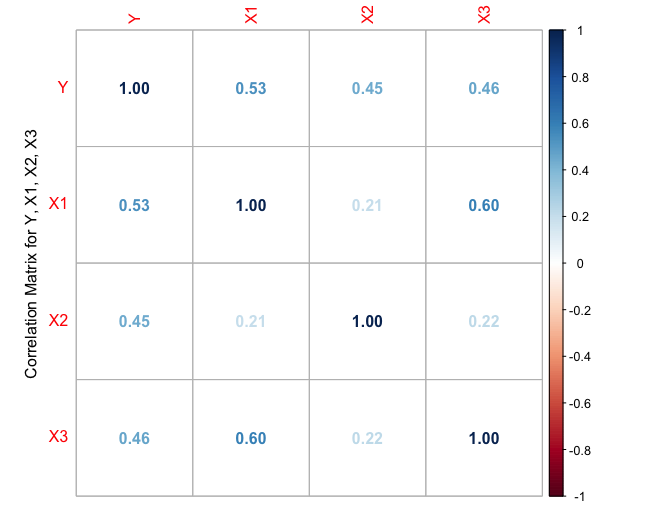
\includegraphics[width=\textwidth]{images/correlationmatrix_question1_part1.png}
          \caption{Correlation Plot bw Variables}
     \end{minipage}%
    \begin{minipage}{.45\textwidth}
       \centering
        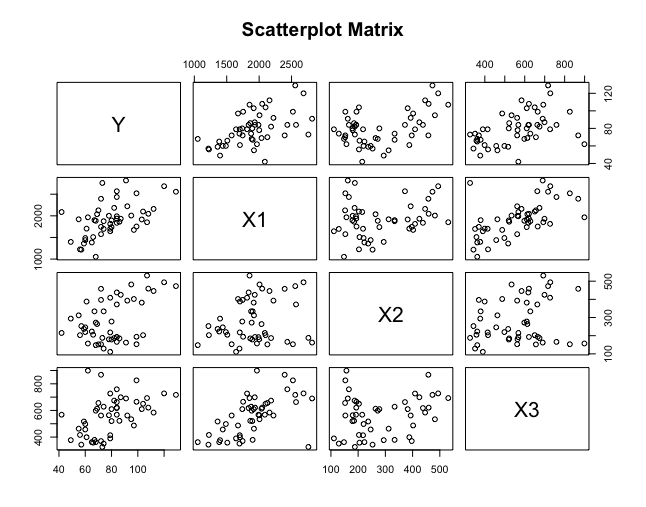
\includegraphics[width=\textwidth]{images/scatterplot_question2_part1.png}
         \caption{Scatter Plot Matrix}
       \end{minipage}
      \end{figure}


The most obvious correlation a variable has with itself, and as we can see from the correlation matrix table (figure 2), each feature variable is highly correlated with itself, indicating a 1:1 linear relationship. 

Moving on to relationships between other variables in figure 2, the first column shows that variable Y (per capita expenditure on shelters/housing in state) has a relatively strong linear relationship with all the features X1, X2 and X3, Y having the strongest relationship with X1. 

In the second row, for X1, the variable is highly correlated with X3, but has a very weak relationship (closer to zero) with X2. 

Additionally, in the same row we can also see that X1 and X3 are the most highly correlated variables in the entire matrix with the highest value of 0.60. This indicates that we have a relationship worth investigating between X1 (per capital personal income in state) with X3 (Number of people/1000 residing in urban areas in state). 

The scatter plots between all variables (figure 3) also show similar patterns to the ones we have in the correlation table. For the relationships that are not strongly dependent (i.e X3 and X2), the data points are scattered, indicating either a non-linear or a non-significant relationship between the two. All other variables that have a decent amount of linear dependence, have data points that cluster alongside (or can be approximated by) a linear line. 
\newpage
\item Part 2

To plot the relationship between Y and Region, I used two different plots. The first figure shows a scatterplot matrix between the variables whereas the second figure shows a boxplot (to be able to find the highest per capita expenditure (on average))


 \begin{figure}[h]
     \centering
       \begin{minipage}{.5\textwidth}
         \centering
           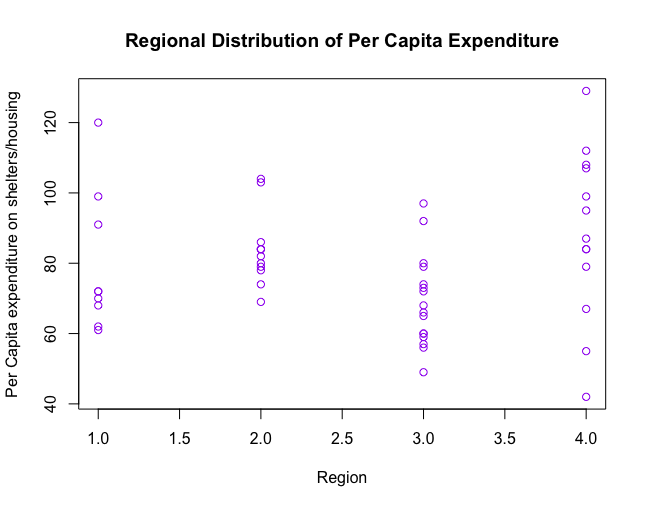
\includegraphics[width=\textwidth]{images/part2_one.png}
          \caption{Scatter Plot Matrix of Regional Distribution of Expenditures}
     \end{minipage}%
    \begin{minipage}{.45\textwidth}
       \centering
        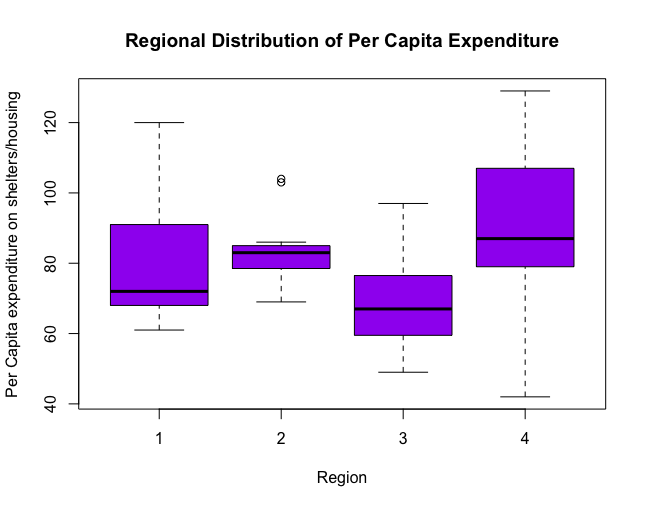
\includegraphics[width=\textwidth]{images/part2_boxplot.png}
         \caption{Box Plot Matrix of Regional Distribution of Expenditures}
       \end{minipage}
      \end{figure}


    On average, region 4 (West) has the highest per capital expenditure on housing assistance. This information is extracted from the fact that Region 4 has the highest median value among all other regions. 

    \newpage

    \item Part 3

     \begin{figure}[h]
     \centering
       \begin{minipage}{.5\textwidth}
         \centering
           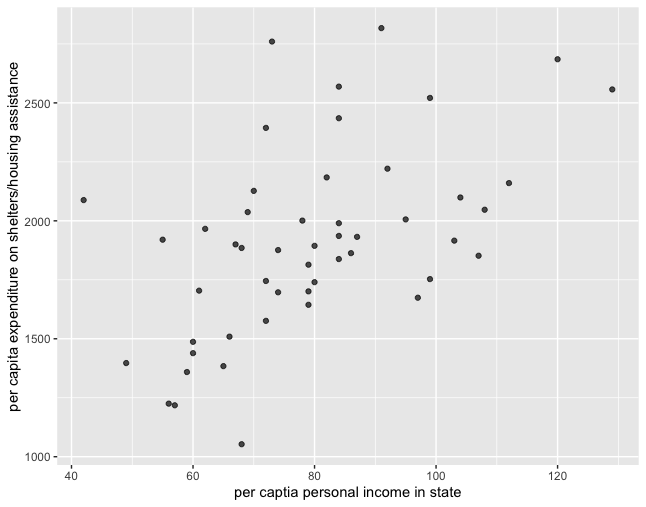
\includegraphics[width=\textwidth]{images/question3_part1.png}
          \caption{Scatter Plot of Y and X1}
     \end{minipage}%
    \begin{minipage}{.45\textwidth}
       \centering
        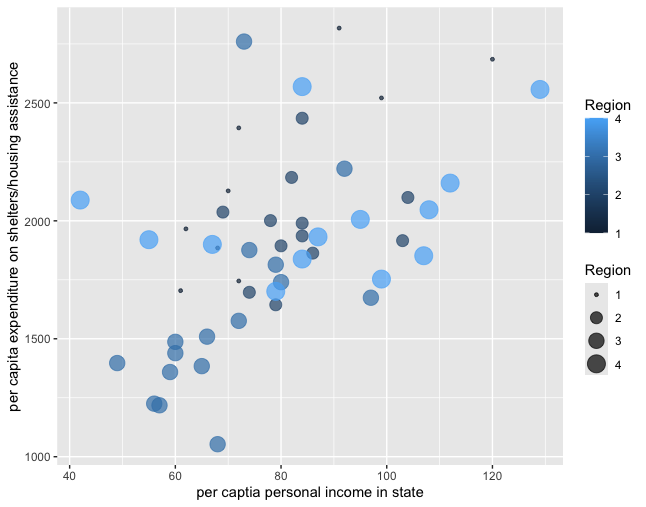
\includegraphics[width=\textwidth]{images/question3_part2.png}
         \caption{Bubble Graph for Y and X1}
       \end{minipage}
      \end{figure}

    As the scatterplot matrix (figure 5) shows Y and X1 have a cluster of data points that can be approximated by a linear line. More points are clustered towards the center diagnally. Its not an ideal 1:1 linear relationship, as we saw in part 1 as well where the two had a correlation factor of 0.53, but it still does appear to be significant. 

    Figure 6 shows the same plot enhanced with a bubble plot where the Region determines the color and the size of the data points. 
\end{enumerate}

\end{document}
